\documentclass{article}
\usepackage{amsmath}
\usepackage{amsfonts}
\usepackage{array}
\usepackage{dsfont}
\usepackage{hyperref}
\usepackage{amssymb}
\usepackage{amsthm}
\usepackage{amsfonts}
\usepackage{graphicx}
% \usepackage{geometry}
\usepackage{bbold}
\usepackage{caption}
% \usepackage{pseudocode}
\usepackage{standalone}
% \usepackage[nottoc]{tocbibind}
% \usepackage{apacite}
\usepackage{etoolbox}
% \usepackage{tikz}
% \usepackage{color}
% \usepackage[T1]{fontenc}
% \usepackage{lmodern}
% \usepackage{mathptmx}
% \usepackage{standalone}
\usepackage{accents}
\usepackage{enumitem}

% used for typesetting theorem environments
\usepackage{amsthm}

% used for typesetting tikz graphs
\usepackage{tikz}
% used for typesetting automata using tikz
\usetikzlibrary{automata}


% aaron edit

%wills stuff


\usepackage{tikz}
\usepackage{algorithmic}
\usepackage{algorithm}
\usepackage{verbatim}
\usepackage[super]{nth}

\graphicspath{ {images/} }

\newcommand{\R}{\mathds{R}}
\newcommand{\Zplus}{\mathds{Z}_+}
\newcommand{\N}{\mathds{N}}
\newcommand{\seq}[2][j]{\left\{#2\right\}_{#1=0}^\infty}
\newcommand{\diff}[3][]{\frac{\mathrm{d}^{#1} #2}{\mathrm{d}^{#1} #3}}
\newcommand{\pdiff}[3][]{\frac{\partial^{#1} #2}{\partial^{#1} #3}}
\newcommand{\dd}{\mathrm{d}}
\newcommand{\ip}[2]{\left\langle #1,#2\right\rangle}
\newcommand{\kernl}[1]{\text{ker}(#1)}
\newcommand{\ind}[1]{\mathbb{1}_{#1}~}
\newcommand{\s}{\mathcal{S}}
\newcommand{\Sin}[1]{\sin\left(#1\right)}
\newcommand{\Cos}[1]{\cos\left(#1\right)}
\newcommand{\ubar}[1]{\underaccent{\bar}{#1}}

\newtheorem{thm}{Theorem}
\newtheorem{assmp}{Assumption}
\newtheorem{prop}{Proposition}
\newtheorem{lemma}{Lemma}

\newcolumntype{C}[1]{>{\centering\arraybackslash}p{#1}}
\newcolumntype{L}[1]{>{\raggedright\arraybackslash}p{#1}}
\newcolumntype{R}[1]{>{\raggedleft\arraybackslash}p{#1}}

\captionsetup[table]{labelfont=bf}
\captionsetup[figure]{labelfont=bf}

\title{Group 5 Thesis}
\author{Us}

\begin{document}
	\maketitle

	\section{Introduction}
		Imagine an object recorded by a camera and represented in a sequence of 2-dimensional, coloured images. The object may change size due to changes in position (closer to the camera) or even by nature (an inflating balloon). The object may enter a shadow or areas with different lighting causing its brightness and colour to change between images. If the object or the camera moves and rotates, then the location of the object, its shape, and even the background of the object will alter over the sequence of images. Nonetheless, a human could view this sequence of images and associate a region in each image as one object being manipulated. 

		Region tracking in a sequence of images seeks to create a computer program that, given a region in an initial image, can identify the region over subsequent images. The tracking is desired to be achieved even if some characteristics of the region change. This report proposes two distinct applications for such a program: hand-gesture tracking and tracking of anatomical structures of CT/MRI scans. While hand-gesture recognition will process images whose sequence represents change in time, the CT/MRI scan will process images whose sequence represents change along a dimension of the 3-dimensional object that was scanned.

		\subsection{Application: Medical Imaging}
			The main imaging modalities chosen were X-ray Computed Tomography (CT) and Magnetic Resonance Imaging (MRI) scans. These modalities were chosen due to their diagnostic performance and ubiquity of use. For surgeons these scans are an integral portion of planning and preparing for procedures. The ability to automatically segment tissues and render models of them in 3D aids in this process and can also be used to produce implants that fit the patient's anatomy to a greater degree.


		\subsection{Application: Gesture Tracking}
			Following a hand through a video sequence can provide individuals with a touchless interface like the Kinect. Using the cheap an ubiquitous web cam the ability to follow gestures can allow a user to interact more fluidly with technology and prevent interruption of some tasks.

	\section{Prob Def}
		Produce an algorithm that efficiently tracks regions in medical and video sequences with low error.

	\section{Math}
		\subsection{Problem Formulation}

		\subsection{Simple Closed Curves}

		\subsection{Level Sets}

		\subsection{Functional Derivations} \label{sec:funcderiv}

	\section{Design}
	The functional pieces described in Section \ref{sec:funcderiv} had to be combined to form complete functionals. These functionals were created based on the invariant properties of the image sets. Of course, medical images and webcam-captured hand gesture images emphasize different invariant properties, thus functionals with different weighting on the functional pieces had to be designed for each application domain.

		\subsection{Medical Images}
		On the medical imaging side of the design, our project focused on high-contrast medical images such as those created by CT scans of bone. On these types of images, we were able to exploit high colour invariance of both the inside and outside of the outlined structure. To capture the colour properties of the images, we needed to heavily weigh inside and outside mean colour. Additionally, we also included the variance property in our functional, although this was weighted to a much weaker extent. The mean colour functional component captured the fact that the average colour on the inside and outside stayed relatively constant between images. The colour variance functional component captured a higher order term for the distribution of the pixel colours. On top of the mean and variance functionals, the length functional was added to stabilize the gradient descent.



		\subsection{Webcam-Generated Hand Gesture Images}
			Faisal

	\section{Implementation}
		Zach

	\section{Results}
		
		\subsection{Final Performance on Medical Images}
		The results of the algorithm using the final optimized parameters are shown in Figures \ref{fig:hip4_25}, \ref{fig:hip4_350}, and \ref{fig:hip4_375}. 
		\begin{figure}[H]
			\centering
			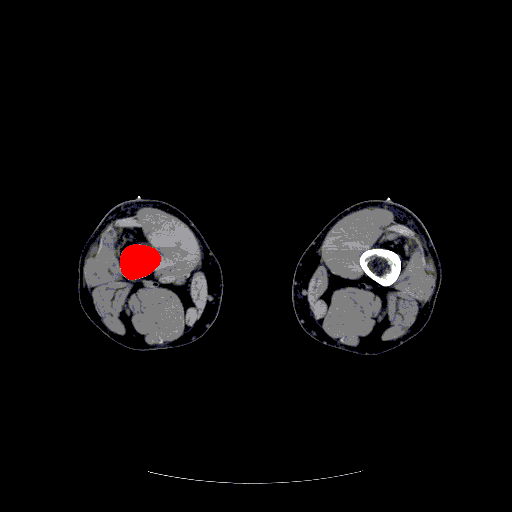
\includegraphics[width=0.4\textwidth]{Hip4/groundTruth25col.png}
			\hspace{20pt}
			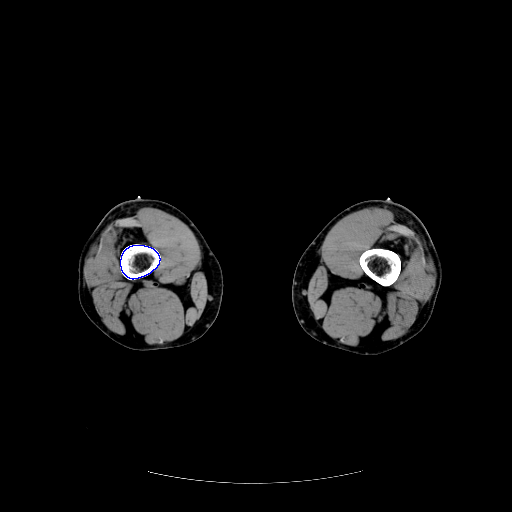
\includegraphics[width=0.4\textwidth]{Hip4/output25.png}
			\caption{Hip image 25 -- ground truth (left) compared to algorithm output with final parameter set (right).}
			\label{fig:hip4_25}
		\end{figure}
		\begin{figure}[H]
			\centering
			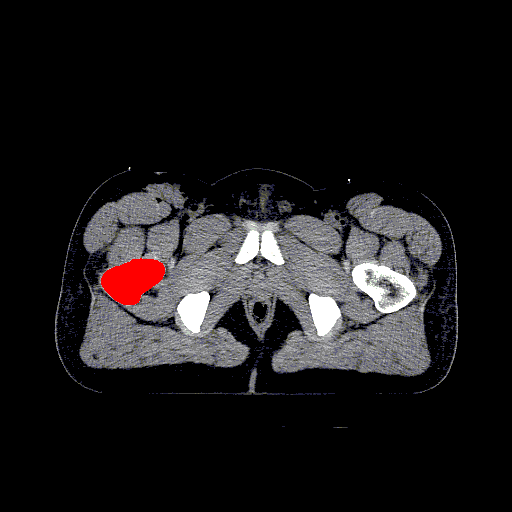
\includegraphics[width=0.4\textwidth]{Hip4/groundTruth350col.png}
			\hspace{20pt}
			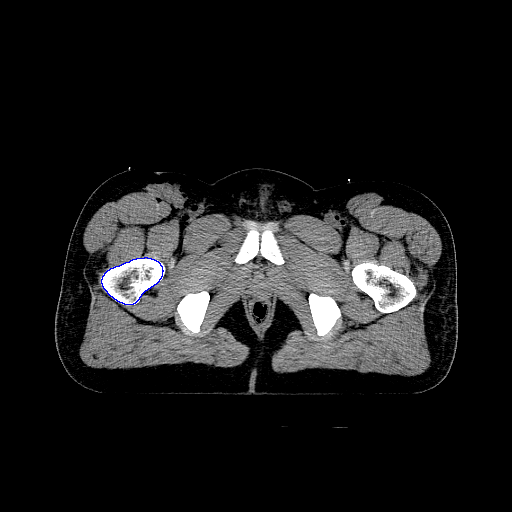
\includegraphics[width=0.4\textwidth]{Hip4/output350.png}
			\caption{Hip image 350 -- ground truth (left) compared to algorithm output with final parameter set (right).}
			\label{fig:hip4_350}
		\end{figure}
		\begin{figure}[H]
			\centering
			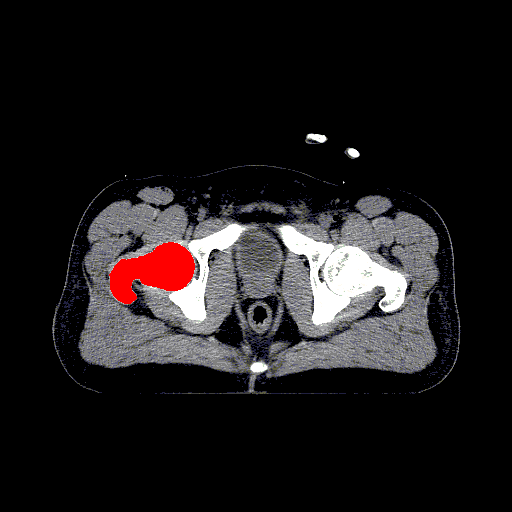
\includegraphics[width=0.4\textwidth]{Hip4/groundTruth375col.png}
			\hspace{20pt}
			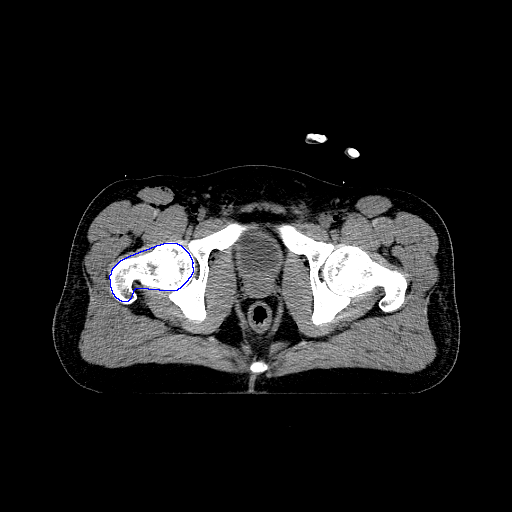
\includegraphics[width=0.4\textwidth]{Hip4/output375.png}
			\caption{Hip image 375 -- ground truth (left) compared to algorithm output with final parameter set (right).}
			\label{fig:hip4_375}
		\end{figure}
		On image 25 (Figure \ref{fig:hip4_25}), the algorithm incorrectly identified 4.13\% of the image pixels by volume of the ground truth. This corresponds to an incorrect identification of 0.017\% of the image pixels over the entire image. As the algorithm proceeded to subsequent images, the error rate did not increase significantly until the shape of the hip bone changed drastically around the \nth{375} image. This is evidenced by the similar error rate obtained in image 350 (Figure \ref{fig:hip4_350}) compared to image 25. In image 350, the percentage of erroneous pixels was 3.82\% of the volume of the ground truth, and 0.041\% of volume of the entire image. However, by image 375 (Figure \ref{fig:hip4_375}), these error rates increased to 13.12\% and 0.17\%, respectively.

		Overall, the algorithm error rate with these final parameters was averaged over the \nth{25}, \nth{75}, \nth{350}, and \nth{375} images. Due to the amount of manual work required to determine ground truth, the evaluation of the algorithm could only be measured over a subset of the images. The images near the beginning and the end of the sequence were assumed to be most revealing of algorithm performance due to gradual shape changes in this dataset. Over this subset, the average error rate as a fraction of ground truth was 6.00\%. The average error rate as a fraction of the entire image was 0.056\%. While we were aiming to have the average error rate over ground truth lower than 5\%, so the algorithm's final performance did not quite reach our expectations in this regard. However, we were also targeting for our algorithm to have less than a 0.1\% error rate over the entire image region, and it outperformed in this metric. See Section \ref{sec:futurework} for areas where the algorithm could have been improved to lower the error rate.
		
		\subsection{Final Performance on Hand Gesture Images}
	\section{Discussion (3bottom)}
		Mandy

	\section{Conclusion}
	\section{Future Work} \label{sec:futurework}
		Faisal
	\nocite{*}
	\bibliographystyle{plain}
	\bibliography{bibliographyExample}
	
\end{document}
